% -------------------------------------------------------------------------------------
% Plantilla de un artículo para publicar en la Revista Colombiana de Estadística
% *************************************************************************************
% -------------------------------------------------------------------------------------
% Establecer primero el idioma principal del artículo, por defecto es español; para
% utilizar otro idioma, cambiar el comando "\documentclass{revcoles}" por el comando
% "\documentclass[english]{revcoles}" o por "\documentclass[portuguese]{revcoles}"
% **** --------------------------------------------------------------------------------
\documentclass[report,oneside]{revcoles}
\usepackage[utf8]{inputenc}
\usepackage[top=2cm,bottom=1cm]{geometry}
\labeldocument[
university = Universidad del Valle,
faculty = Facultad de Ingeniería,
department = Escuela de Estadística,
program = Programa Académico de Estadística,
subject = Análisis Multivariante,
city = Cali,
month = 9,
year = 2018]

% -------------------------------------------------------------------------------------
% Espacio reservado para la carga de los paquetes por parte del autor
% **** --------------------------------------------------------------------------------




% //// --------------------------------------------------------------------------------
% -------------------------------------------------------------------------------------
% Espacio reservado para colocar las definiciones especiales por parte del autor
% **** --------------------------------------------------------------------------------



% //// --------------------------------------------------------------------------------
% -------------------------------------------------------------------------------------
% Espacio utilizado para colocar las palabras que necesitan partición silábica
% **** --------------------------------------------------------------------------------
\hyphenation{Colombia mul-ti-va-ria-do pro-ba-bi-li-dad es-ta-dís-ti-ca}
% //// --------------------------------------------------------------------------------
\begin{document}

% -------------------------------------------------------------------------------------
% Espacio reservado para ingresar el título del artículo
% "maintitle = " título original del artículo
% "secondtitle = " título del artículo traducido al idioma alterno
% "shorttitle = " título corto (opcional) para el encabezado
% **** --------------------------------------------------------------------------------
\title[maintitle = {Laboratorio 2: Análisis de Componentes Principales },
       %secondtitle = Template for report in a course,
       shorttitle = Análisis de Componentes Principales 
]
% //// --------------------------------------------------------------------------------
% -------------------------------------------------------------------------------------
% Espacio reservado para ingresar el(los) autor(es) del artículo de forma individual.
% opción "firstname = " nombres completos de cada autor
% opción "surname = " primer apellido de cada autor
% opción "numberinstitution = " número que identifica la institución a la que pertenece
%         el autor, en caso de haber solo una institución el campo se elimina
% opción "affiliation = " afiliación o cargo que desempeña el autor en la institución
% opción "email = " dirección electrónica del autor (preferiblemente institucional)
% **** --------------------------------------------------------------------------------
\begin{authors}
\author[firstname = Kevin Steven,
        surname = García,
        code = Código: 1533173,
        email = kevin.chica@correounivalle.edu.co,
]
\author[firstname = Alejandro,
        surname = Vargas,
        code = Código: 1525953 ,
        email = jose.alejandro.vargas@correounivalle.edu.co
]
\author[firstname = Alejandro,
        surname = Soto,
        code = Código: 1532457 ,
        email = asotomurillo@gmail.com
]
\end{authors}
% //// --------------------------------------------------------------------------------
% -------------------------------------------------------------------------------------
% Espacio reservado para ingresar la información de la(s) institución(es) a la(s)
% cual(es) pertenece(n) el(los) autor(es)
% Usar un comando "\institute"  por cada una de las diferentes instituciones.
% Los campos "subdivision" y "division" son opcionales
% Los campos "institution", "city" y "country" son obligatorios
% **** --------------------------------------------------------------------------------
\begin{comment}
\begin{institutions}
     \institute[subdivision = Departamento de Estadística,
                division = Facultad de Ciencias,
                institution = Universidad del Valle,
                city = Cali,
                country = Colombia]
\end{institutions}
\end{comment}
% //// --------------------------------------------------------------------------------
% -------------------------------------------------------------------------------------
% CUERPO DEL DOCUMENTO
% **** --------------------------------------------------------------------------------
% -------------------------------------------------------------------------------------
% Espacio reservado para colocar el resumen en el idioma principal y las palabras clave
% !!No dejar salto de línea entre el resumen y el comando \keywords{.}¡¡
% **** --------------------------------------------------------------------------------
\begin{comment}
\begin{mainabstract}
Este documento contiene las instrucciones de presentación de los
trabajos de cursos. Este texto está escrito utilizando \LaTeX\
como editor según formato adjunto (archivo \emph{Template for Report.tex})
y puede utilizarse como guía, reemplazando este contenido. Se requieren los
archivos \emph{revcoles.cls}, \emph{references.bib} y \emph{graph\_example.eps}.%
%
\keywords{Formato en \LaTeX\ para documentos, carrera de Estadística}
\end{mainabstract}
\end{comment}
% //// --------------------------------------------------------------------------------
% -------------------------------------------------------------------------------------
% Espacio reservado para colocar el resumen en el idioma secundario y las palabras clave
% !!No dejar salto de línea entre el resumen y el comando \keywords{.}¡¡
% **** --------------------------------------------------------------------------------
\begin{comment}
\begin{secondaryabstract}
This document gives the instructions to prepare a \LaTeX\ version of the graduation project of undergraduate in
Statistics to first semester of 2008. The document is written using a \LaTeX\ format (file \emph{Plantilla para trabajo
de grado.tex}) and can be used as a guideline just replacing its contents. It is necessary to use also the files
\emph{revcoles.cls}, \emph{references.bib} and \emph{graph\_example.eps}.
%
\keywords{\LaTeX\ format for documents, undergraduate in Statistics}
\end{secondaryabstract}

\end{comment}% //// --------------------------------------------------------------------------------
% -------------------------------------------------------------------------------------
% Título de la primera sección
% **** --------------------------------------------------------------------------------
\section{Introducción}
~\\En este informe se llevará a cabo el análisis de componente principales a una base de datos correspondiente a la ``Encuesta de Presupuestos Familiares del año 1990/91'' en España. esta se cuenta con 51 observaciones y 9 variables. Las observaciones son las provincias españolas más Ceuta y Melilla, que aparecen unidas como una única provincia, y las variables son:$X_1$= alimentación, $X_2$= vestido y calzado, $X_3$= vivienda, $X_4$= moviliario doméstico, $X_5$= gastos sanitarios, $X_6$= transporte, $X_7$= enseñanza y cultura, $X_8$= turismo y ocio, $X_9$= otros gastos. En este análisis se tomará en cuenta conceptos como el análisis exploratorio de los datos, la nube de individuos y de variables (circulo de correlaciones), la representación simultanea, la construcción e interpretación del indice, los cosenos cuadrados y las contribuciones y las relaciones de transición.

\section{Análisis exploratorio}
~\\En el análisis exploratorio vamos a realizar un análisis descriptivo y gráfico para cada variable y se obtendrá la matriz de correlaciones para posteriormente realizar comparaciones con los resultados del ACP.
\begin{itemize}
\item Estadísticas descriptivas

\begin{figure}[h!]
  \centering
  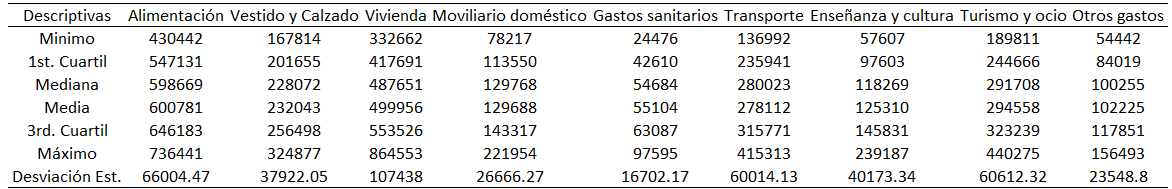
\includegraphics[scale=0.52]{FigurasUV/desc.png}
\end{figure}

~\\En esta tabla podemos ver las estadísticas descriptivas de los presupuestos familiares de cada provincia española para las variables medidas. Se puede observar que en cuanto a los promedios, como es de esperarse, las provincias destinan en general, mas dinero de su presupuesto en la alimentación, con un promedio de 600781 euros por provincia para las familias, seguido de los presupuestos para vivienda, que son en promedio de 499956 euros por provincia. En cambio, a lo que menos destinan dinero las provincias es en gastos sanitarios, con un promedio de 55104 euros. El presupuesto máximo que tuvo una provincia fue para gastos familiares en vivienda, con un presupuesto destinado de 864553 euros y el presupuesto mínimo, fue precisamente para gastos sanitarios, con un presupuesto de solo 24476. En cuanto a la variación de los presupuestos entre provincias. Las provincias tienen presupuestos menos variables en los gastos sanitarios, con una desviación estándar de solo 16702.17 euros, lo contrario sucede con los gastos en vivienda, donde cada provincia tiene gastos o presupuestos muy variables en este aspecto, presenta una desviación estándar de 107438 euros.
\begin{figure}[h!]
  \centering
  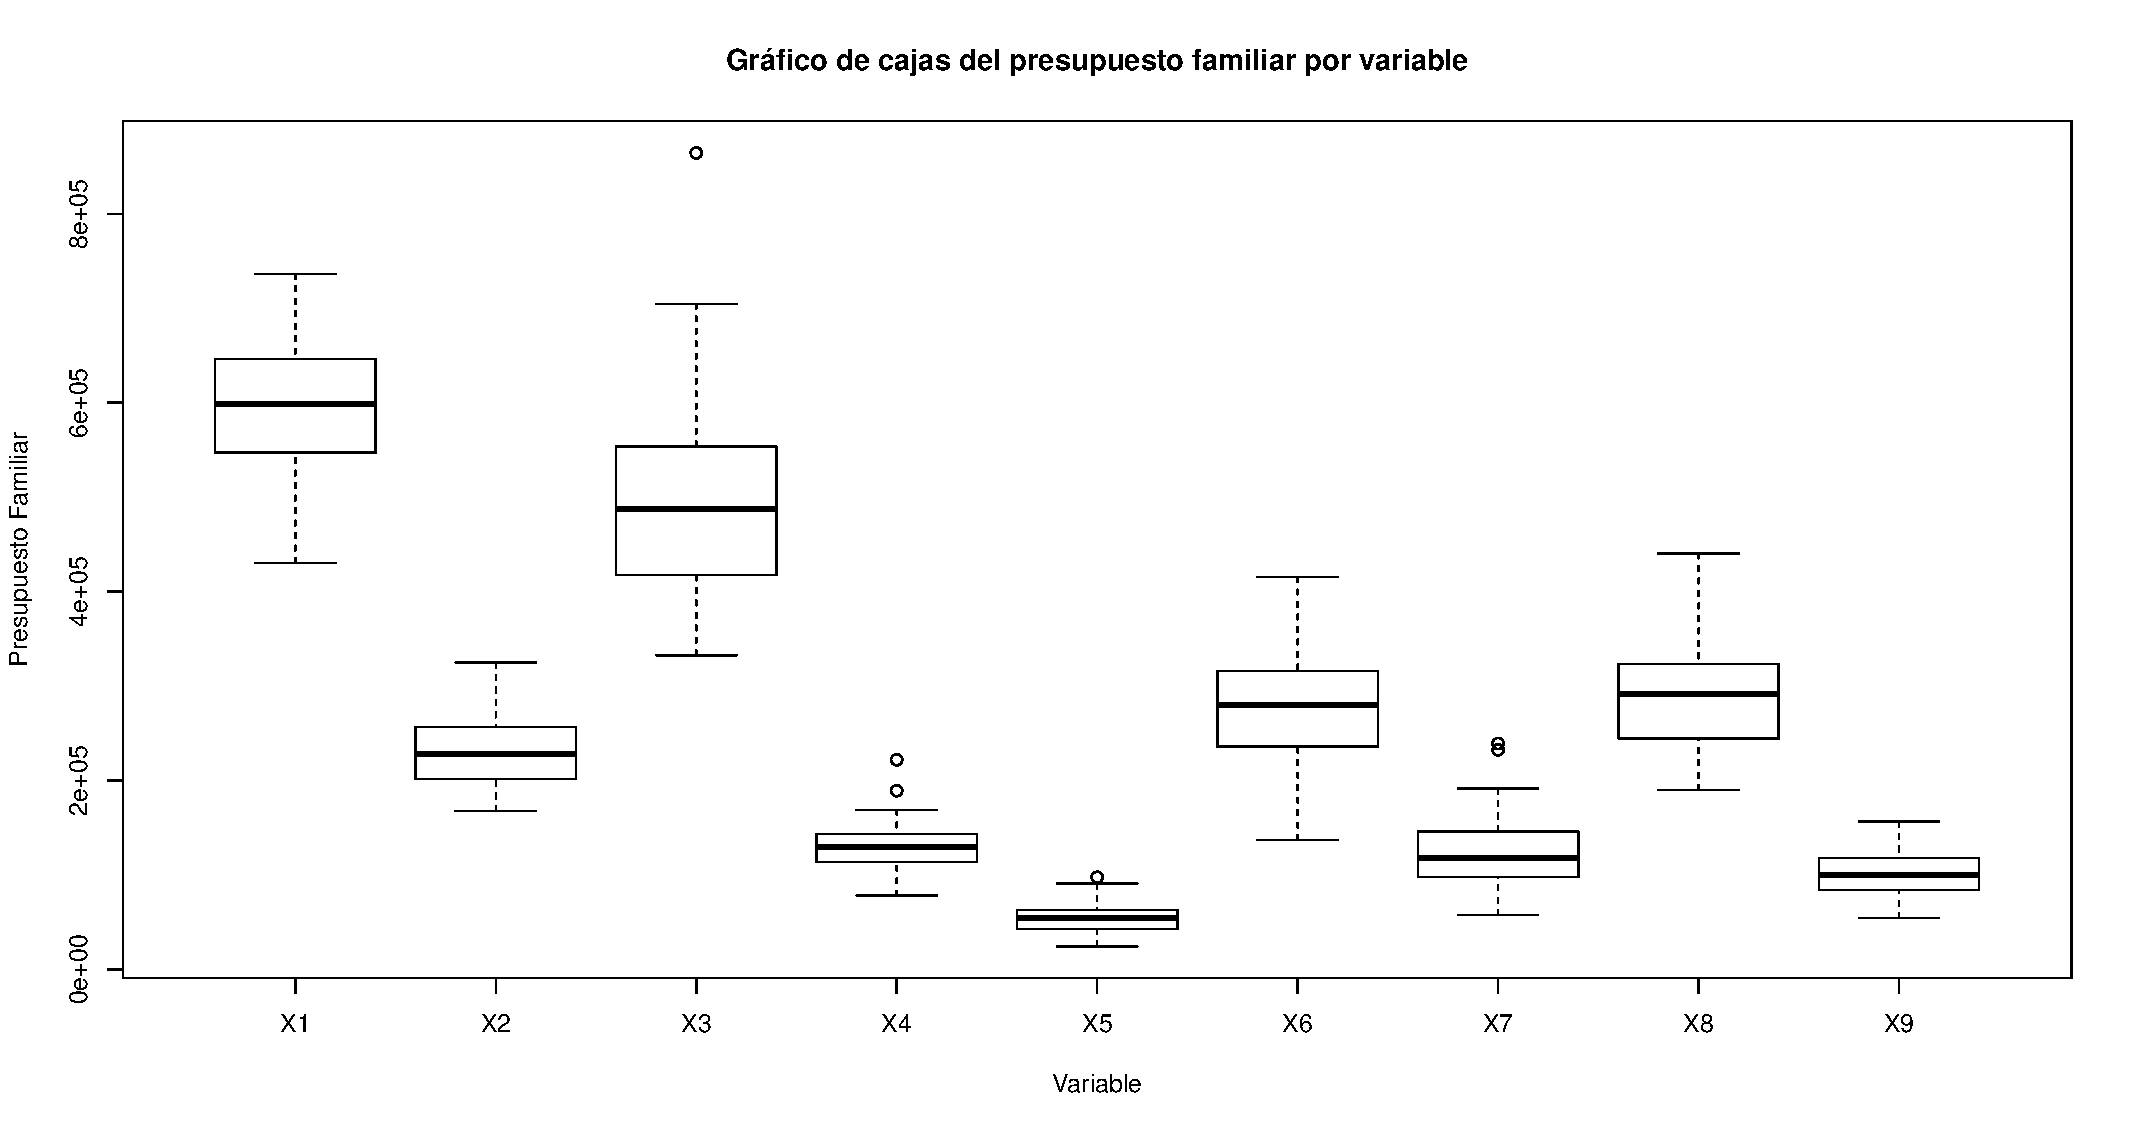
\includegraphics[scale=0.45]{FigurasUV/cajas.pdf}
\end{figure}

~\\En esta gráfica podemos confirmar las interpretaciones dadas anteriormente. Se puede observar que en promedio los presupuestos de las provincias para los gastos familiares en alimentación ($X_1$) y vivienda ($X_3$) son mucho mayores que el resto. En los presupuestos familiares para vivienda, vemos un punto atípico muy alto, que corresponde a una provincia que tiene un presupuestos para ello de 864553 euros (fue el mayor presupuesto de todos). Podemos observar que los presupuestos para gastos familiares correspondientes a $X_2$ (Vestido y calzado),$X_6$ (Transporte) y $X_8$ (Turismo y ocio) se comportan de manera parecida en las provincias en cuanto a su promedio y a su variabilidad, es un poco menor y menos variable los presupuestos familiares en vestido y calzado. Finalmente, los menores presupuestos de las provincias corresponden a las variables $X_4$,$X_5$,$X_7$ y $X_8$, donde evidenciamos en todas estas variables (excepto $X_9$) algunos puntos atípicos (no muy graves) por encima.

\item Matriz de correlaciones
\begin{center}
\resizebox{15cm}{!} {
\begin{tabular}{cccccccccc}
 
 & X1 & X2 & X3 & X4 & X5 & X6 & X7 & X8 & X9\\ 

X1 & 1 &0.531518& 0.475464& 0.516663& 0.474304& 0.527562& 0.588739& 0.438100& 0.483185 \\ 

X2 & 0.531518 &1& 0.549165& 0.633367& 0.505310& 0.587491& 0.545900& 0.462608& 0.532391 \\ 
 
X3 & 0.475464& 0.549165& 1& 0.698918& 0.670385& 0.691356& 0.833379& 0.810211& 0.541736 \\ 

X4 & 0.516663 &0.633367 &0.698918 &1 &0.674083 &0.727259 &0.755607 &0.756133 &0.635271 \\ 

X5 & 0.474304 &0.505311 &0.670385& 0.674083& 1& 0.729750& 0.812126& 0.705834 &0.590650 \\ 

X6 & 0.527562 &0.587492 &0.691356 &0.727259 &0.729750 &1 &0.744703 &0.726837 &0.713231 \\ 

X7 & 0.588739 &0.545900& 0.833379& 0.755607& 0.812126& 0.744703 &1& 0.844991& 0.562388 \\ 
 
X8 & 0.438100 &0.462608 &0.810211 &0.756133 &0.705834 &0.726837 &0.844991 &1 &0.582652 \\ 

X9 & 0.483185 &0.532391& 0.541736& 0.635271& 0.590650& 0.713231& 0.562388& 0.582652& 1 \\ 

\end{tabular}
} 
\end{center}
\end{itemize}
~\\En la matriz de correlaciones podemos ver correlaciones altas en las variables $X_3$ con $X_7$ y $X_8$ con 0.8334 y 0.8102 respectivamente. También vemos una correlación alta entre $X_5$ y $X_7$ con 0.8121 y entre $X_7$ y $X_8$ con 0.845. Se espera que esto se vea evidenciado en la nube de las variables, es decir, que la representación de estas variables con altas correlaciones sea muy cercana en el gráfico. Si no somos tan estrictos en las correlaciones, se podría decir que todas las variables se correlacionan fuertemente, ya que la mínima correlación entre las variables es la de $X_1$ y $X_8$ con una correlación de 0.4381. Entonces podemos afirmar que todas las variables están correlacionadas positivamente, por lo que esperamos que en la nube de variables, todas tengan el mismo sentido o signo, y no estén tan alejadas.


\pagebreak
\section{Porcentaje de Inercia y ejes seleccionados}
\begin{center}
\begin{tabular}{|c|c|c|c|}
\hline 
 & Valor propio & Porcentaje de varianza & Porcentaje de varianza acumulada \\ 
\hline 
comp 1 & 6.08732572     &         67.636952&                          67.63695\\
comp 2 &0.77720888     &          8.635654  &                        76.27261\\
comp 3 &0.55666880    &           6.185209   &                       82.45782\\
comp 4 &0.47914455   &            5.323828    &                      87.78164\\
comp 5 &0.34768511  &             3.863168     &                     91.64481\\
comp 6 &0.27435674 &              3.048408      &                    94.69322\\
comp 7 &0.22712456&               2.523606       &                   97.21683\\
comp 8 &0.15329446&               1.703272        &                  98.92010\\
comp 9 &0.09719117&               1.079902         &                100.00000 \\
\hline 
\end{tabular} 
\end{center}

\begin{figure}[h!]
  \centering
  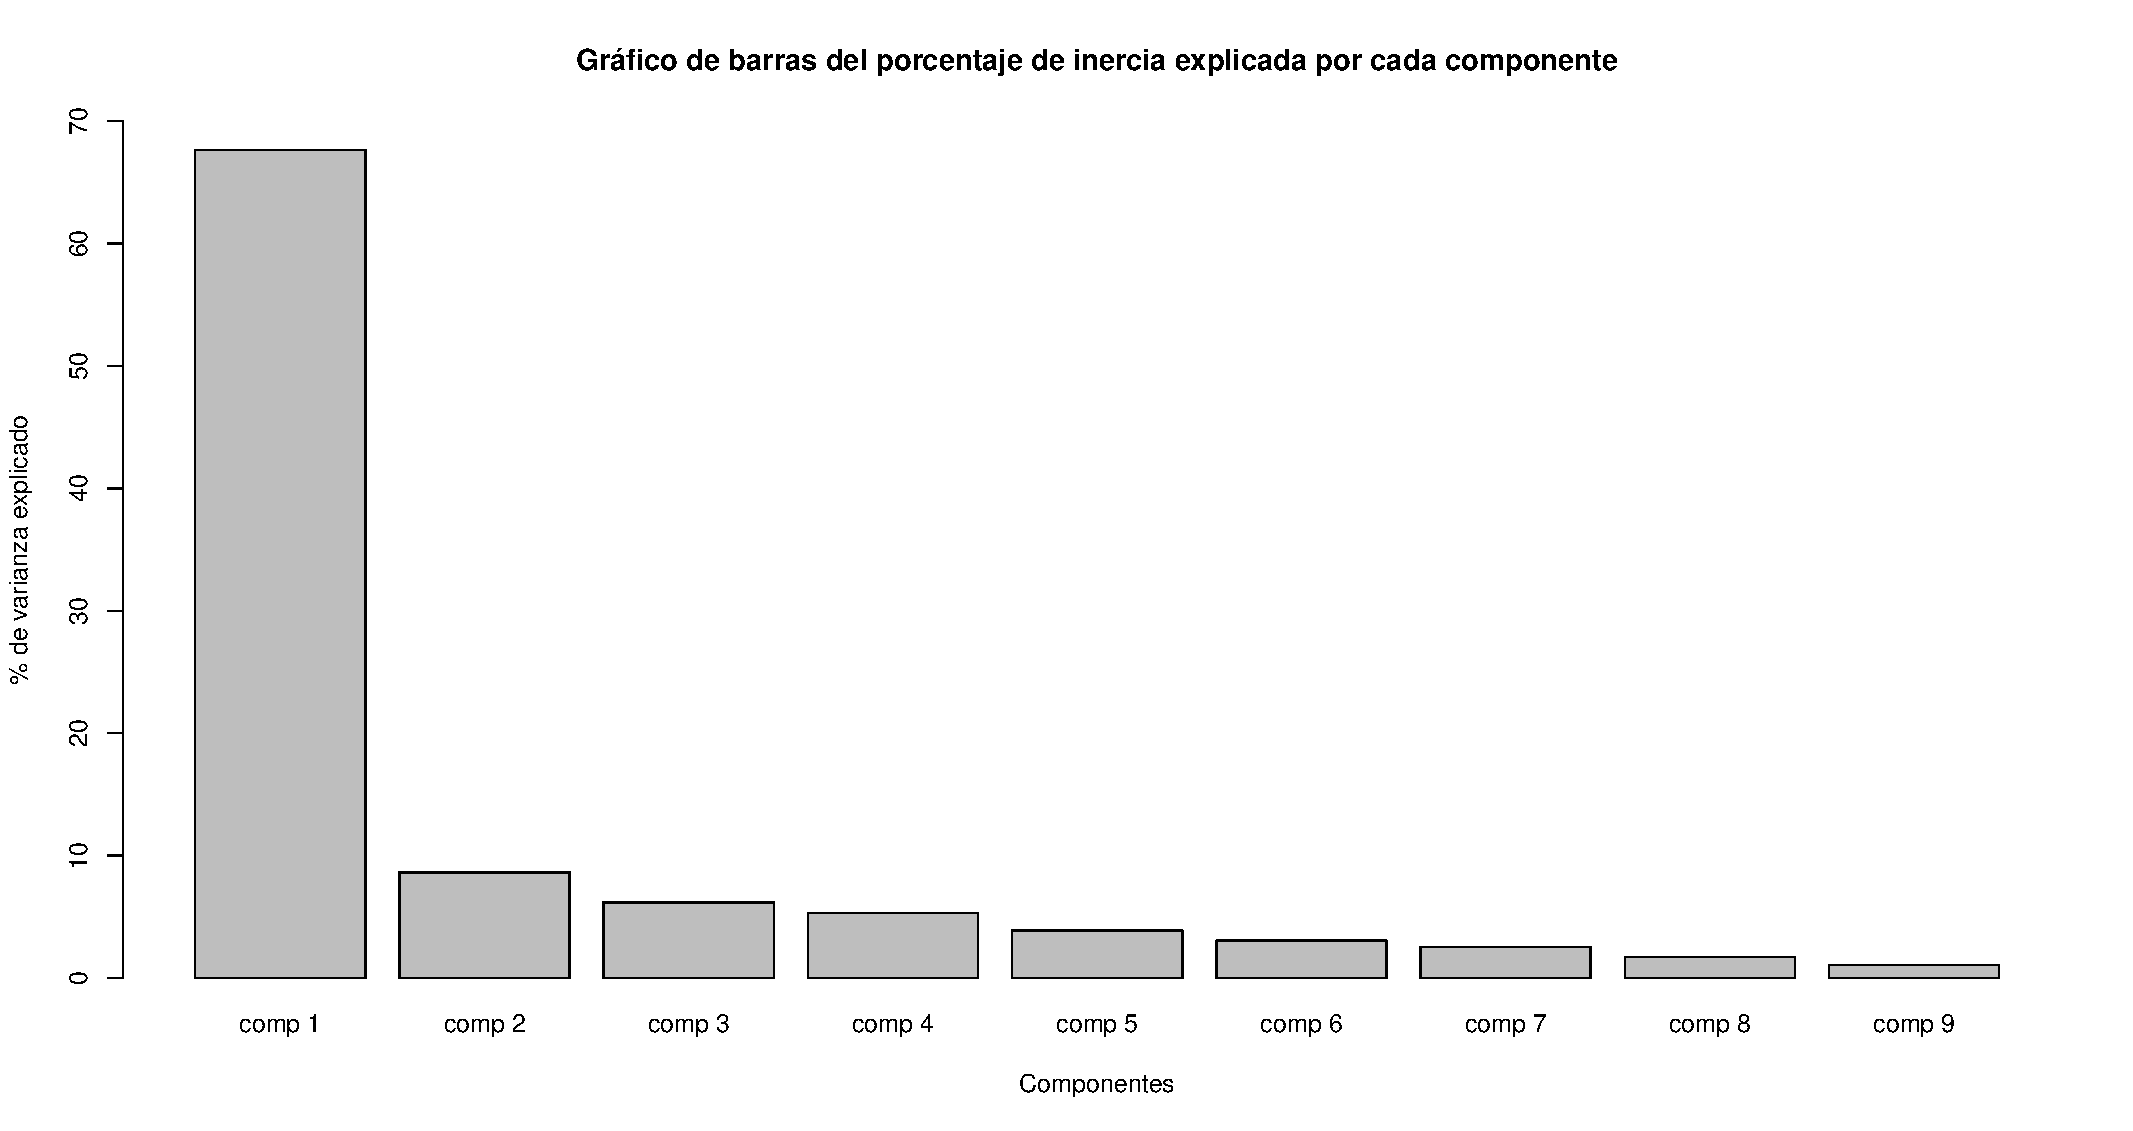
\includegraphics[scale=0.45]{FigurasUV/varianza.pdf}
\end{figure}

~\\En la tabla y la gráfica anterior, vemos el porcentaje de varianza explicado por cada componente, observamos que con las primeras dos componentes, se acumula un 76.27 \% de varianza explicada, y el aumento de la componente 3, no es muy significativo, por lo cuál optamos por utilizar las dos primeras componentes.

\section{Resultados ACP}
\subsection{Valores propios}
~\\Los valores propios obtenidos fueron

\begin{center}
\resizebox{17cm}{!} {
\begin{tabular}{|ccccccccc|}
\hline 
$\lambda_1$ & $\lambda_2$ & $\lambda_3$ & $\lambda_4$ & $\lambda_5$ & $\lambda_6$ & $\lambda_7$ & $\lambda_8$ & $\lambda_9$ \\ 
6.08732572 & 0.77720888 & 0.55666880 & 0.47914455 & 0.34768511 & 0.27435674 & 0.22712456  & 0.15329446 & 0.09719117 \\ 
\hline 
\end{tabular} 
}
\end{center}
\pagebreak
\subsection{Vectores propios: Variables}
~\\Los dos primeros vectores propios para las variables fueron

\begin{center}
\begin{tabular}{|c|c|c|}
\hline 
Variable & v1 & v2 \\ 
\hline 
$X_1$ & 0.2695709 & 0.581576684 \\ 
$X_2$ & 0.2885398 & 0.535194871 \\  
$X_3$ & 0.3476300 & -0.274191765 \\  
$X_4$ & 0.3528739 & -0.002137995 \\  
$X_5$ & 0.3410886 & -0.199767613 \\  
$X_6$ & 0.3555715 & 0.007846322 \\ 
$X_7$ & 0.3705182 & -0.229288381 \\  
$X_8$ & 0.3521639 & -0.389951665 \\  
$X_9$ & 0.3076265 & 0.235680269 \\ 
\hline 
\end{tabular} 
\end{center}

\subsection{Componentes: Variables}
~\\Las dos primeras componentes para las variables fueron:

\begin{center}
\begin{tabular}{|c|c|c|}
\hline 
Variable & c1 & c2 \\ 
\hline 
$X_1$ & 0.6650990  & 0.512714812 \\ 
$X_2$ & 0.7119000 &  0.471824861\\  
$X_3$ & 0.8576904 & -0.241725956 \\  
$X_4$ & 0.8706285 &  -0.001884845\\  
$X_5$ & 0.8415510 &  -0.176114032\\  
$X_6$ & 0.8772839 &  0.006917274\\ 
$X_7$ & 0.9141612 & -0.202139378 \\  
$X_8$ & 0.8688766 & -0.343779248  \\  
$X_9$ & 0.7589916 & 0.207774432 \\ 
\hline 
\end{tabular} 
\end{center}

\section{Nube de individuos}
\begin{figure}[h!]
  \centering
  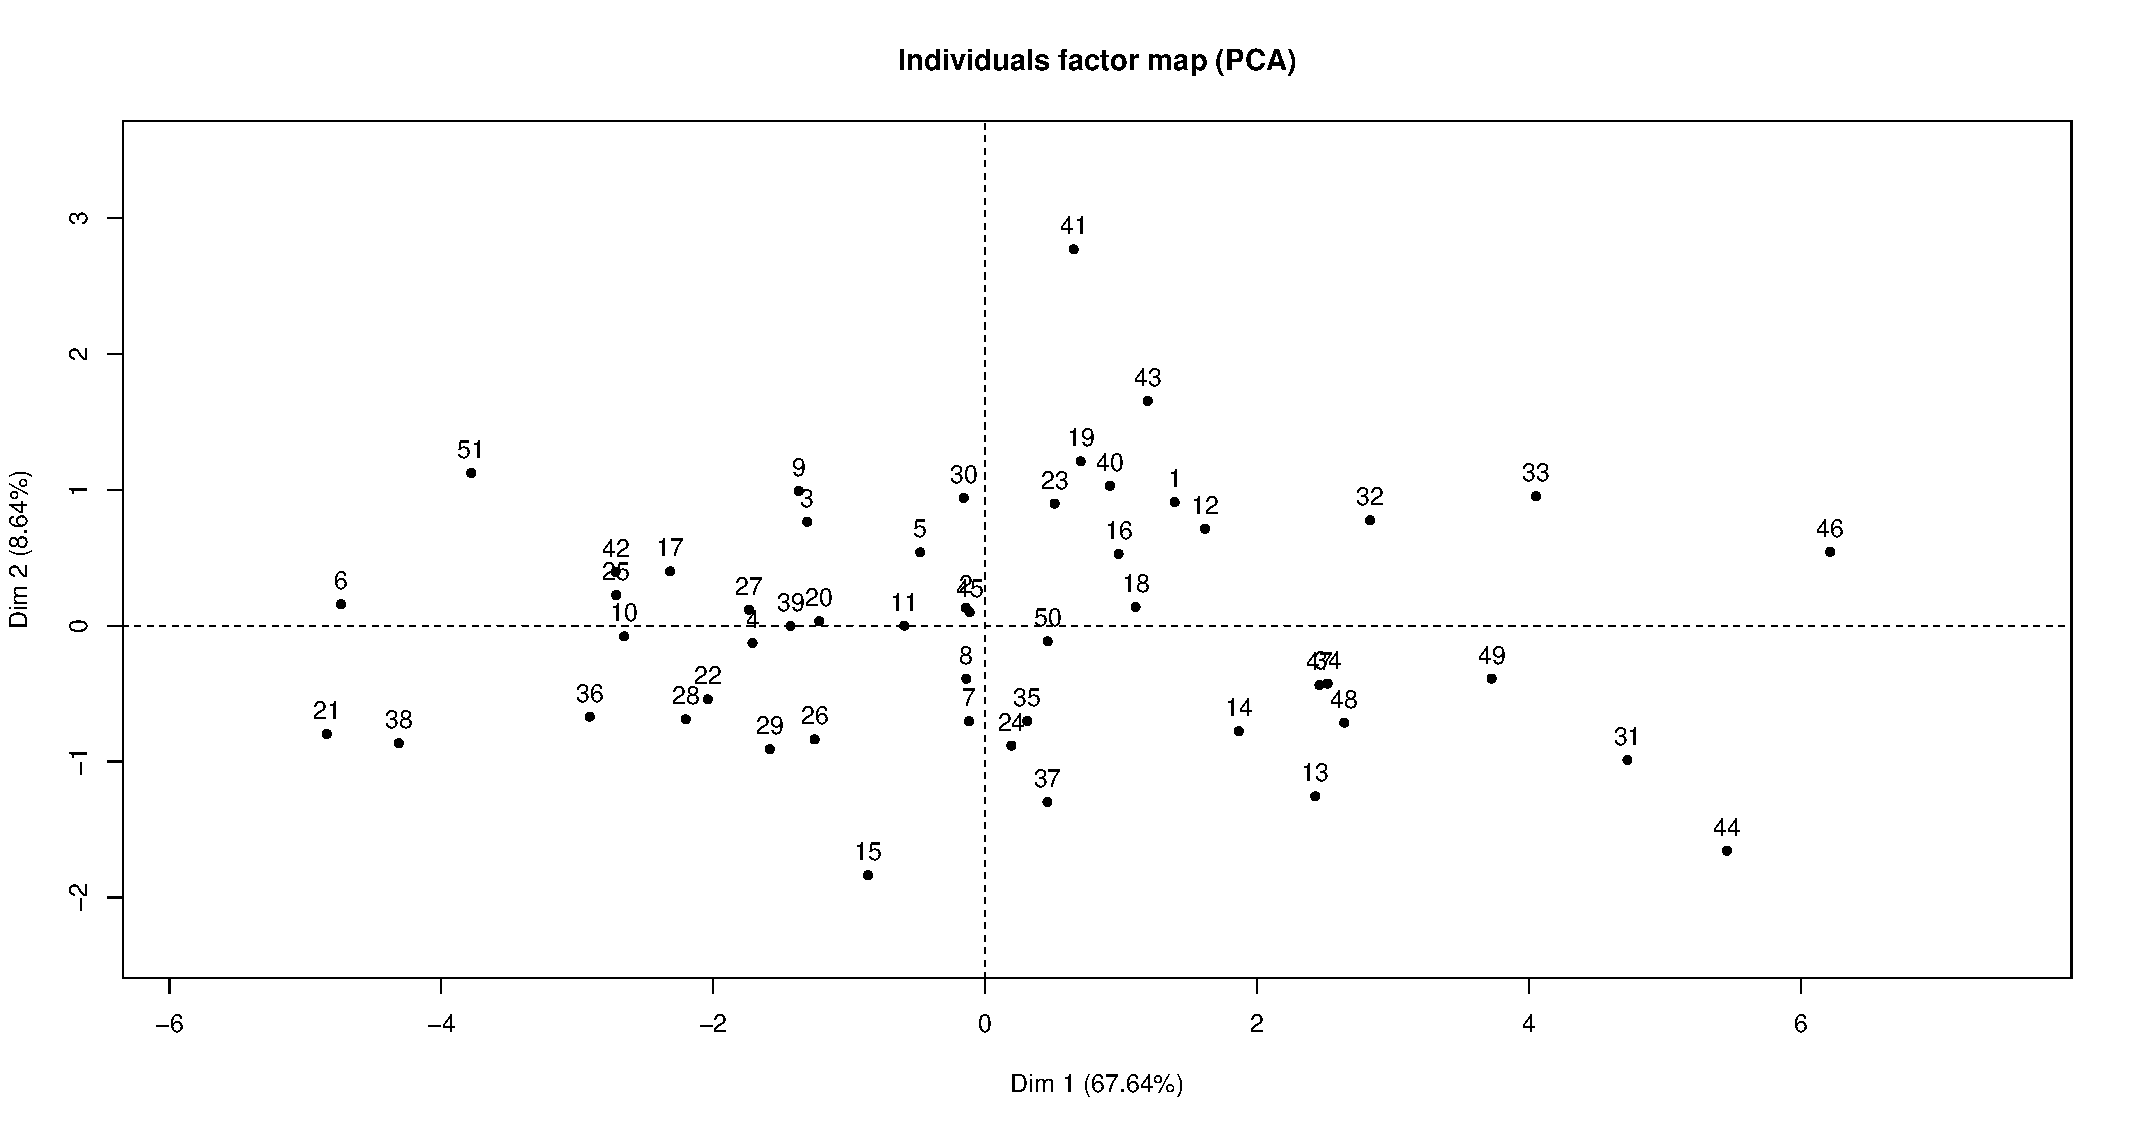
\includegraphics[scale=0.45]{FigurasUV/nubeind.pdf}
\end{figure}
~\\Sobre esta nube de individuos no se puede dar fácilmente una interpretación clara, ya que son muchos individuos. Lo que se puede evidenciar es que una gran parte de las provincias españolas están muy cercanas en cuanto a los gastos o presupuestos familiares en las 9 variables medidas. Hay excepciones y casos especiales de provincias donde sus gastos fueron muy alejados del resto. Posteriormente se dará una mejor interpretación en la representación simultanea.

\section{Circulo de correlaciones}
\begin{figure}[h!]
  \centering
  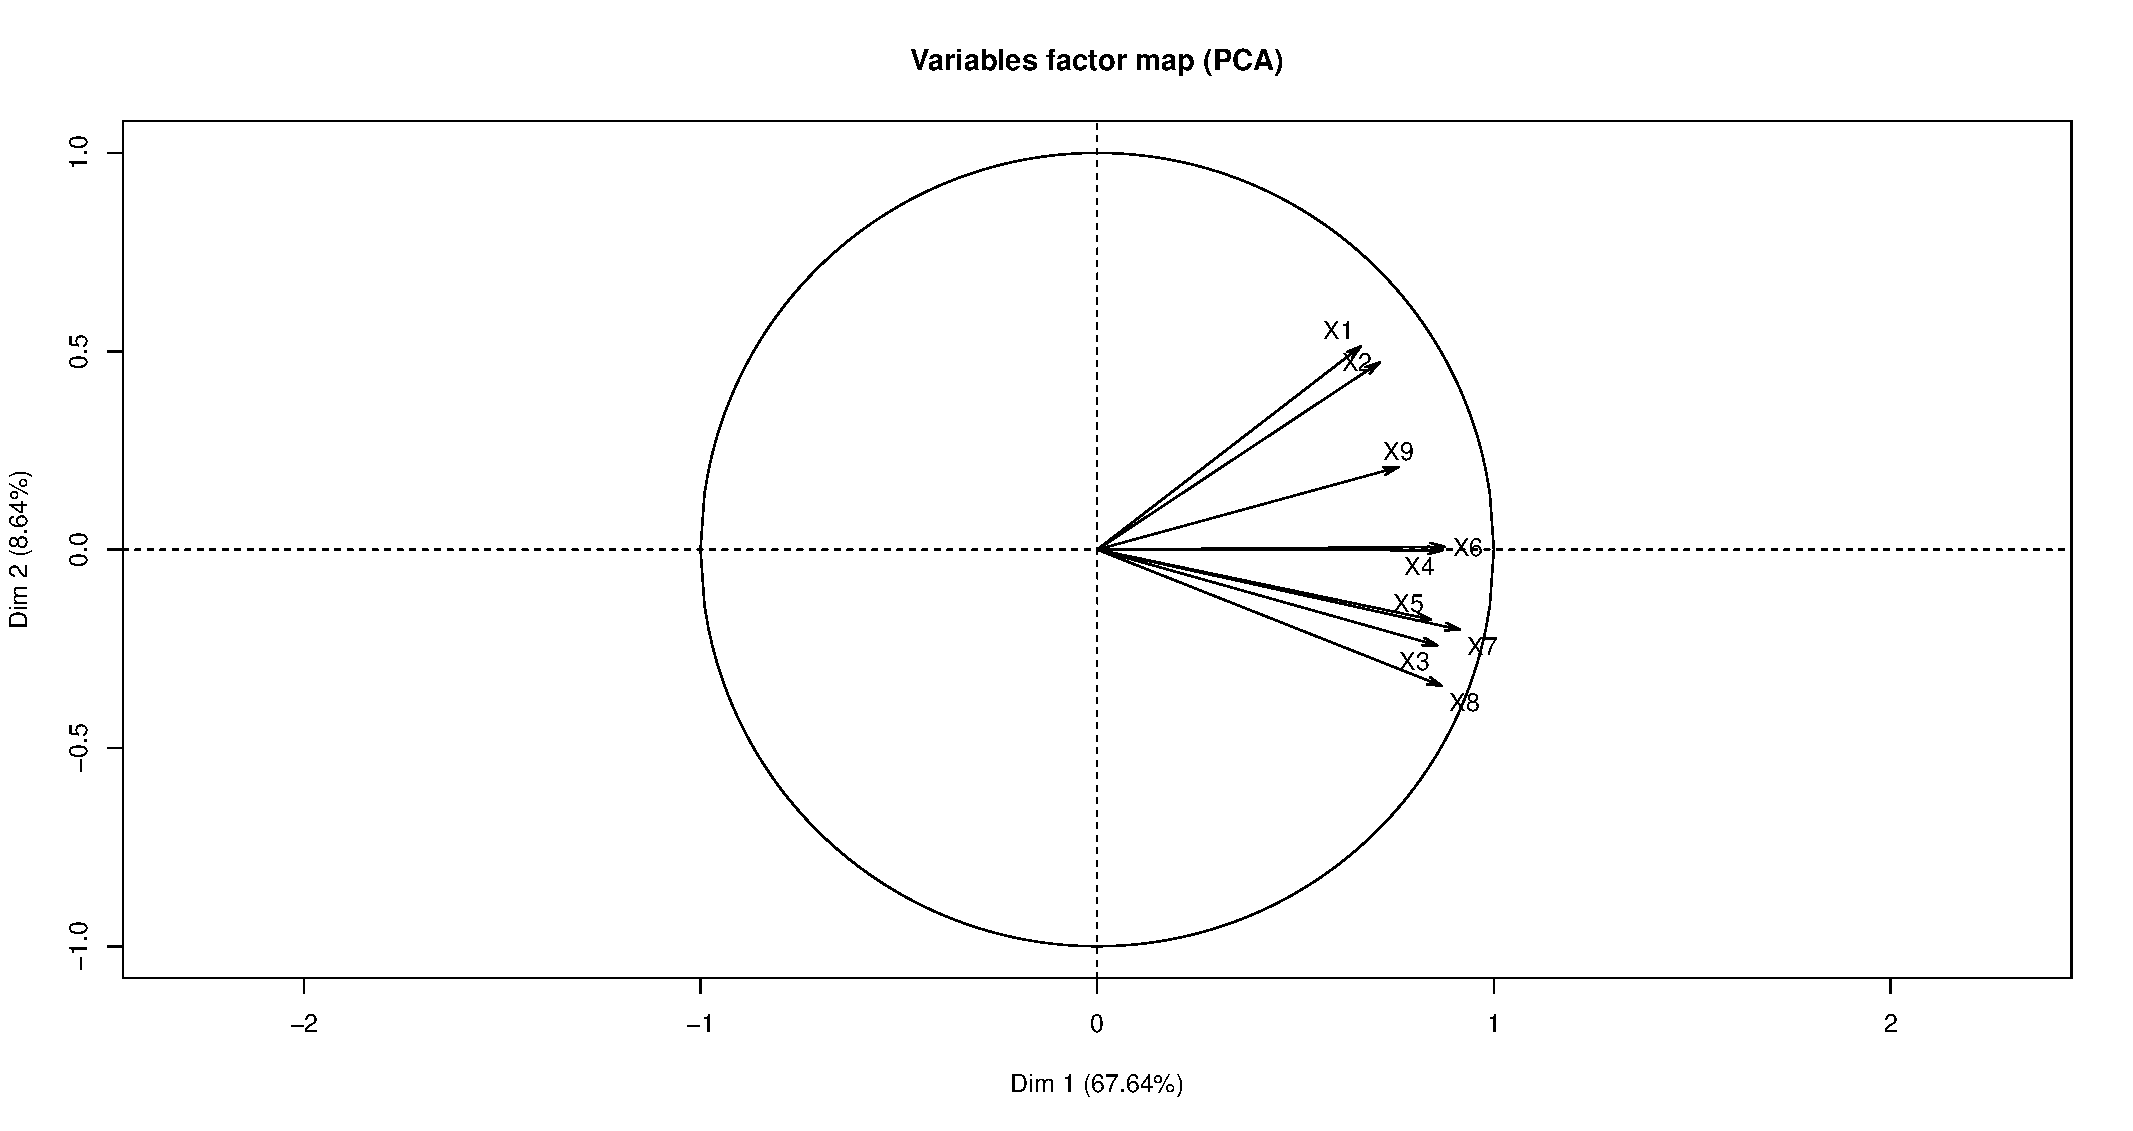
\includegraphics[scale=0.45]{FigurasUV/nubevar.pdf}
\end{figure}

~\\En esta gráfica que corresponde al circulo de correlaciones, podemos ver que aparentemente todas las 9 variables están bien representadas por estas dos componentes y la mayoría contribuyen de manera similar a la construcción del eje 1, esto se verificara más adelante con los cosenos cuadrados y las contribuciones. Además se corrobora las hipótesis que teníamos inicialmente de la matriz de correlaciones (que todas las variables iban a estar cercanas la una de la otra, y que todas iban a tener el mismo sentido).

\section{Representación simultanea}
\begin{figure}[h!]
  \centering
  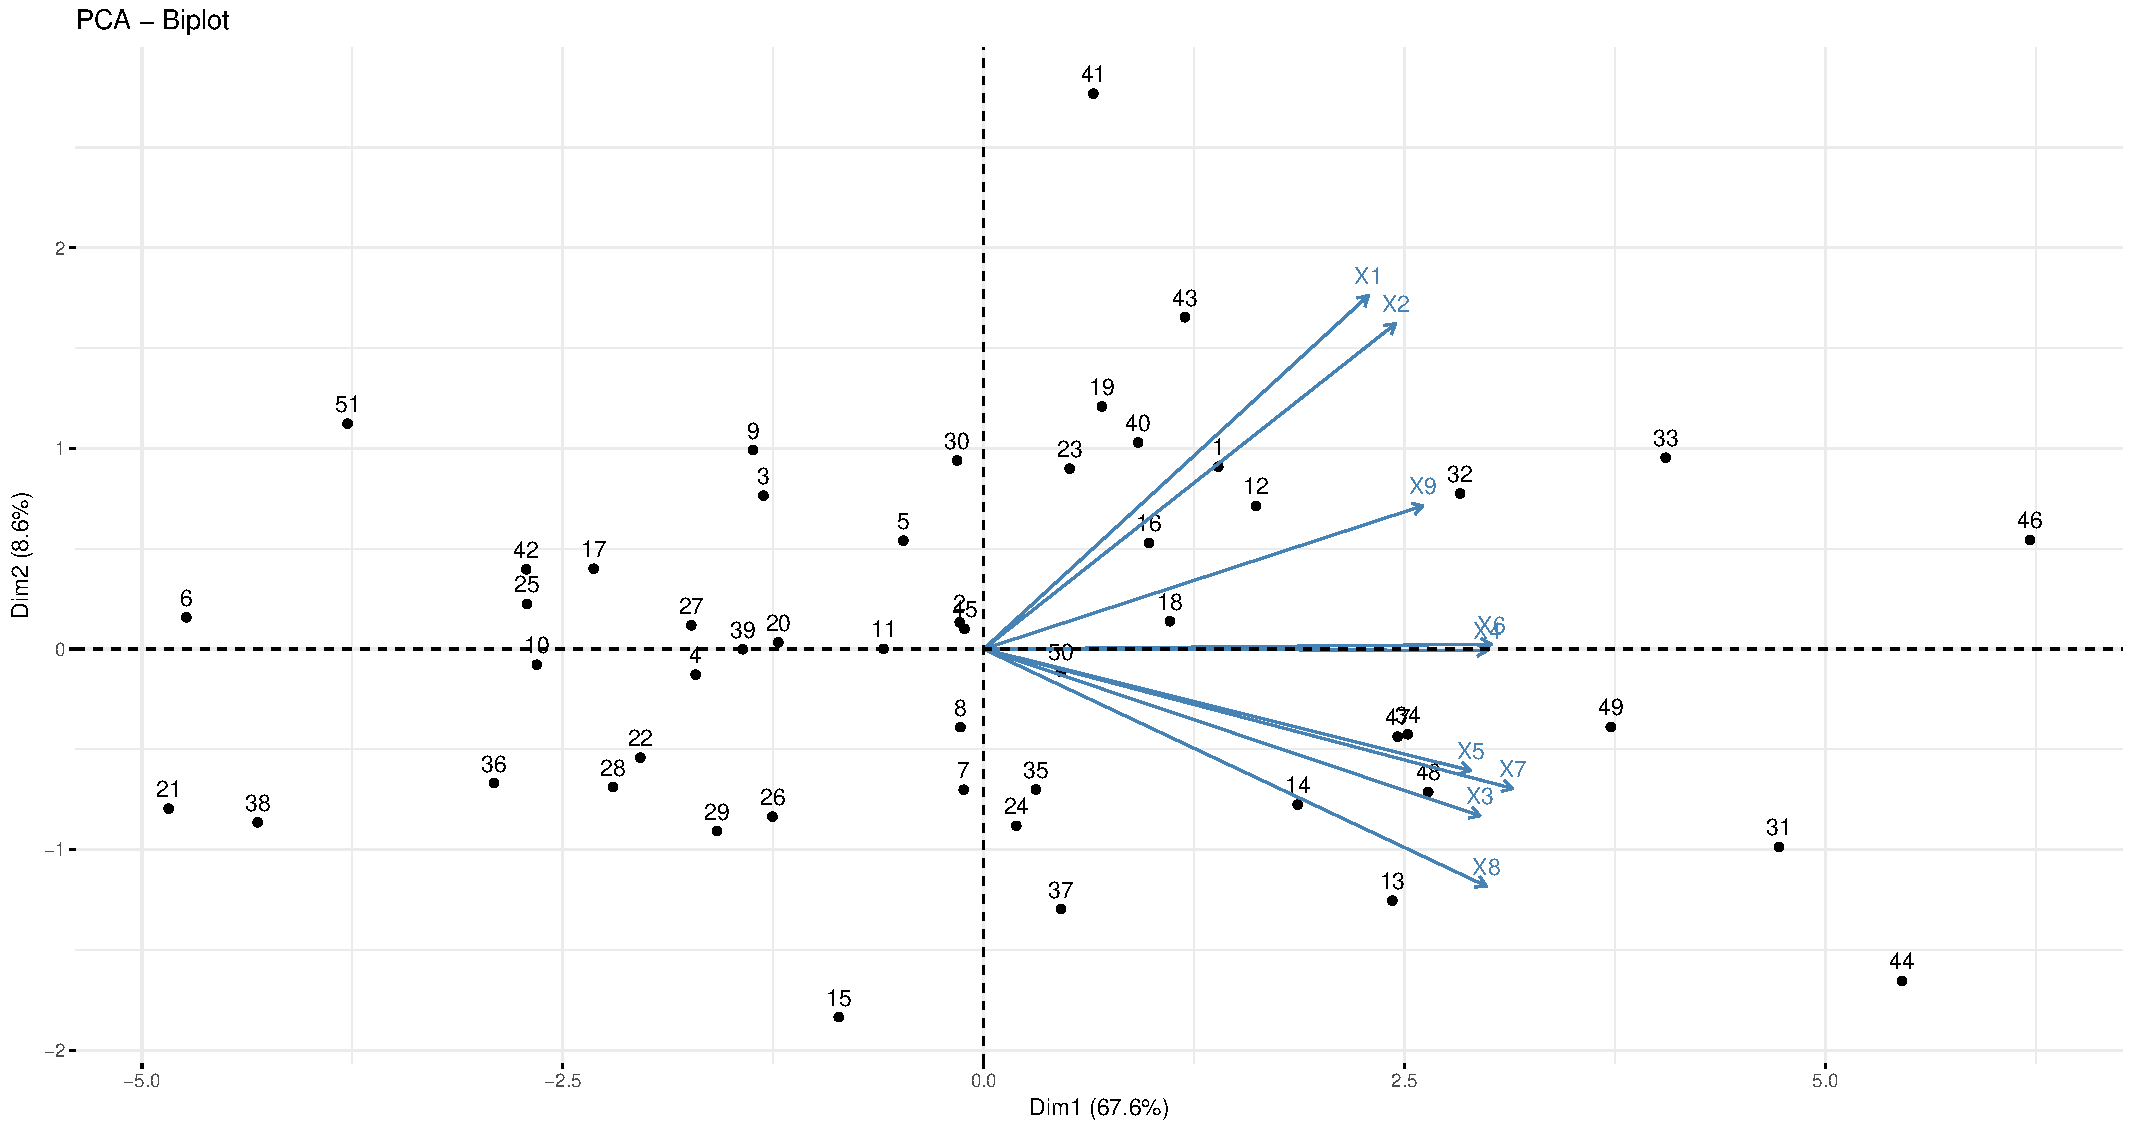
\includegraphics[scale=0.45]{FigurasUV/biplot.pdf}
\end{figure}

~\\En esta gráfica se puede observar, que hay muchas provincias donde los gastos familiares son muy bajos en varias de las variables medidas, por ejemplo, las provincias 6 (Jaén),21 (Salamanca),38 (Badajoz) y 51 (Ceuta y Melilla) tienen valores muy bajos en casi todas las variables, esto nos dice que las familias que pertenecen a estas provincias, probablemente no tengan tantos recursos para gastar en estos aspectos y se podría analizar  la calidad de vida de estas familias, en cambio, hay provincias que tienen altos valores en cuanto al presupuesto familiar en algunas o todas estas variables, como por ejemplo, las provincias 46 (Navarra),44 (Madrid),31 (Barcelona),32 (Gerona),33 (Lérida),49 (Vizcaya), entre otras. Se puede observar que aparecieron provincias importantes como Navarra, Madrid y Barcelona, era de esperarse ya que en estas provincias las familias tienen una mejor calidad de vida en general que las familias de otras provincias, por lo que los presupuestos y los gastos familiares en estas provincias, van a ser mayores en todas las variables.

\pagebreak
\section{Contribuciones y cosenos cuadrados}
~\\Los cosenos cuadrados y las contribuciones de las variables en las tres primeras dimensiones o componentes son:
\begin{center}
\begin{tabular}{|c|cc|cc|}
\hline 
 Variable &Cosenos & Cuadrados  &  Contribuciones  &   \\ 
 &Componente 1 & Componente 2  & Componente 1 & Componente 2 \\ 
X1 &0.4423566& 0.2628765& 7.266847& 33.82314 \\
X2 &0.5068016 & 0.2226187& 8.325522& 28.64335 \\
X3 &0.7356329 &0.0584314& 12.084665& 7.518112 \\
X4 &0.7579939 &0.0000035 & 12.452002& 0.0004571 \\
X5 &0.7082081 &0.0310161 & 11.634141& 3.990710 \\
X6 &0.7696271 &0.00004785& 12.643107& 0.0061565 \\
X7 &0.8356907 &0.0408603& 13.728371& 5.257316 \\
X8 &0.7549465 &0.1181842& 12.401940& 15.20623 \\
X9 &0.5760683 &0.0431702& 9.463405& 5.554519 \\
\hline 
\end{tabular} 
\end{center}

~\\En la tabla anterior, con respecto a los cosenos cuadrados. Podemos ver que en la primera componente, la variable $X_7$ (Enseñanza y cultura) es la que esta mejor representada con un coseno cuadrado de 0.8357 y la variable $X_1$ (alimentación) es la que menos representada esta por esta componente, con un coseno cuadrado de 0.4423. Pero en general, se podría decir que la mayoría de variables esta bien representada por esta componente. Observando la componente 2, las únicas que están aceptablemente representadas son las variables $X_1$ y $X_2$ (Vestido y calzado) con cosenos cuadrados de 0.2629 y 0.2226 respectivamente.

~\\Centrándonos en las contribuciones, observamos que con respecto a la primera componente, como se esperaba (por el circulo de correlaciones), casi todas las variables contribuyen de igual forma a la construcción del primer eje, la que más contribuye es $X_7$ (Enseñanza y cultura) con una contribución de 13.7284 y la que menos contribuye es $X_1$ (alimentación) con una contribución de 7.2668. En cuanto a la segunda componente, las variables ya no contribuyen de forma parecida a la construcción del eje 2, las que mas contribuyen son $X_1$, $X_2$ y $X_8$ con contribuciones de 33.82, 28.64 y 15.21 respectivamente.

\section{Indice}
~\\Para darnos cuenta si se puede realizar el indice, nos debemos fijar en el circulo de correlaciones y observar si se cumple el factor tamaño, es decir, que todas las variables tengan el mismo sentido con respecto al eje 1, esto también se podría ver en los signos del primer vector propio, ya que este define el signo de las coordenadas, si todos los signos del primer vector propio son iguales, podemos construir un indice con la primera componente principal. En este caso, podemos observar que todos los signos del primer vector propio son positivos y en el circulo de correlaciones, que todas las variables van en el mismo sentido con respecto al eje 1, por lo que tenemos lo que se denomina como factor tamaño y se puede realizar la construcción del indice.

~\\Con la primera componente principal, se realiza la construcción del indice:

\begin{center}
\begin{tabular}{|c|c|}
\hline 
Variable & Componente 1 \\ 
\hline 
$X_1$ & 0.6650990 \\ 
$X_2$ & 0.7119000 \\  
$X_3$ & 0.8576904 \\ 
$X_4$ & 0.8706285 \\ 
$X_5$ & 0.8415510 \\ 
$X_6$ & 0.8772839 \\ 
$X_7$ & 0.9141612 \\  
$X_8$ & 0.8688766 \\ 
$X_9$ & 0.7589916 \\ 
\hline 
\end{tabular} 
\end{center}

~\\El indice es:

$$I=0.6650990 X_1 +0.7119000 X_2 + 0.8576904 X_3 + 0.8706285 X_4 + 0.8415510 X_5+ 0.8772839 X_6 +$$
$$0.9141612 X_7 + 0.8688766 X_8 + 0.7589916 X_9$$

~\\El cuál lo podríamos denominar como indice de presupuestos familiares, tendríamos un indice para cada provincia, entonces lo que se esperaría, es que los que tengan un valor mas alto en este indice, son las provincias  que tienen un mayor desarrollo y sus habitantes tienen una mejor calidad de vida. Por ejemplo se espera que los indices de Madrid, Navarra y Barcelona, sean de los más altos según las interpretaciones anteriores.

\section{Puntos Adicionales}
\subsection{Relaciones de transición}
~\\La descomposición con la función svd() de R, a la matriz $N^{\frac{1}{2}}Z$, donde N es la matriz con $\frac{1}{51}$ en su diagonal, es la siguiente:

~\\Los valores propios son:
\begin{center}
\resizebox{17cm}{!} {
\begin{tabular}{|ccccccccc|}
\hline 
$\lambda_1$ & $\lambda_2$ & $\lambda_3$ & $\lambda_4$ & $\lambda_5$ & $\lambda_6$ & $\lambda_7$ & $\lambda_8$ & $\lambda_9$ \\ 
2.4672506 & 0.8815945 & 0.7461024 & 0.6922027 & 0.5896483 & 0.5237907 & 0.4765759 & 0.3915284 & 0.3117550 \\ 
\hline 
\end{tabular} 
}
\end{center}

~\\Los vectores propios para las variables son:
\begin{center}
\begin{tabular}{|c|c|c|}
\hline 
Variable & v1 & v2 \\ 
\hline 
$X_1$ & 0.2695709 & 0.581576684 \\ 
$X_2$ & 0.2885398 & 0.535194871 \\  
$X_3$ & 0.3476300 & -0.274191765 \\  
$X_4$ & 0.3528739 & -0.002137995 \\  
$X_5$ & 0.3410886 & -0.199767613 \\  
$X_6$ & 0.3555715 & 0.007846322 \\ 
$X_7$ & 0.3705182 & -0.229288381 \\  
$X_8$ & 0.3521639 & -0.389951665 \\  
$X_9$ & 0.3076265 & 0.235680269 \\ 
\hline 
\end{tabular} 
\end{center}

~\\Podemos ver que esta función nos saca los mismos vectores propios que en el ACP, pero los valores propios son distintos, exactamente son la raíz cuadrada de los valores propios que nos arroja el ACP.

~\\Las relaciones de transición son $\Psi_\alpha=\sqrt{\lambda_\alpha} N^{-\frac{1}{2}} v_\alpha$  \;\; y \;\;   $\varphi=\sqrt{\lambda_\alpha}u_\alpha$ 
~\\En la siguiente tabla se verán las dos primeras componentes para las variables con esta relación de transición 
\begin{center}
\begin{tabular}{|c|c|c|}
\hline 
Variable & c1 & c2 \\ 
\hline 
$X_1$ & 0.4234281  & 0.546061334 \\             
$X_2$ & 0.4532234 &  0.502511936\\  
$X_3$ & 0.5460393 & -0.257447600 \\  
$X_4$ & 0.5542762 &  -0.002007433\\  
$X_5$ & 0.5357643 &   -0.187568334\\  
$X_6$ & 0.5585133 &   0.007367167\\   
$X_7$ & 0.5819908 & -0.215286346 \\  
$X_8$ & 0.5531609 & -0.366138348   \\  
$X_9$ & 0.4832038 & 0.221287899 \\ 
\hline 
\end{tabular} 
\end{center}

~\\Se puede observar que la relación no funciona, ya que no obtenemos las componentes principales, en las componentes para los individuos también ocurre lo mismo, pero como se menciono anteriormente, los valores propios obtenidos de esta matriz con la función svd(), son la raíz cuadrada de los valores propios obtenidos del ACP o de la función eigen() a la matriz de correlaciones. por lo cuál, para que nos arroje los verdaderos componentes, las relaciones de transición deben ser:
$$\Psi_\alpha=\lambda_\alpha N^{-\frac{1}{2}} v_\alpha$$
$$\varphi=\lambda_\alpha u_\alpha$$

~\\Se le quita la raíz a los valores propios.
~\\Con esta relación se obtienen las siguientes dos primeras componentes para las variables
\begin{center}
\begin{tabular}{|c|c|c|}
\hline 
Variable & c1 & c2 \\ 
\hline 
$X_1$ & 0.6650990  & 0.512714812 \\ 
$X_2$ & 0.7119000 &  0.471824861\\  
$X_3$ & 0.8576904 & -0.241725956 \\  
$X_4$ & 0.8706285 &  -0.001884845\\  
$X_5$ & 0.8415510 &  -0.176114032\\  
$X_6$ & 0.8772839 &  0.006917274\\ 
$X_7$ & 0.9141612 & -0.202139378 \\  
$X_8$ & 0.8688766 & -0.343779248  \\  
$X_9$ & 0.7589916 & 0.207774432 \\ 
\hline 
\end{tabular} 
\end{center}

~\\Las cuales si son las componentes originales. Lo mismo ocurre con las componentes de los individuos, esta relación si nos da las componentes dadas por el ACP.

\subsection{Varianza de las componentes en el espacio de las variables}
~\\la varianza de cada componentes $v(\varphi)$ en el espacio de las variables se muestran en la siguiente tabla
\begin{center}
\resizebox{17cm}{!} {
\begin{tabular}{|ccccccccc|}
\hline 
$v(\varphi_1)$ & $v(\varphi_2)$ & $v(\varphi_3)$ & $v(\varphi_4)$ & $v(\varphi_5)$ & $v(\varphi_6)$ & $v(\varphi_7)$ & $v(\varphi_8)$ & $v(\varphi_9)$ \\ 
0.006485077 & 0.085682921 & 0.061845612 & 0.053234137 & 0.038631116 & 0.030475913 & 0.025223868 & 0.017030272 & 0.010791507 \\ 
\hline 
\end{tabular} 
}
\end{center}


\section{Conclusión}
~\\Con respecto al ACP realizado, observamos que las familias que tienen mayor presupuesto para los gastos en las 9 variables medidas, son las pertenecientes a las provincias de Madrid, Barcelona, Navarra, Vizcaya, Lérida y Gerona; por lo que se podría decir que la calidad de vida que tienen las personas en estas provincias es mucho mayor que la calidad de vida de las familias pertenecientes a las demás provincias.




% //// --------------------------------------------------------------------------------
% -------------------------------------------------------------------------------------
% Fin del cuerpo del documento
% **** --------------------------------------------------------------------------------
% **** --------------------------------------------------------------------------------
% Espacio para colocar el nombre del archivo *.bib (sin la extensión .bib) que contiene
% las referencias bibliográficas del artículo utilizando el estilo bibliográfico BibTeX
% "\referencias{.}"
% **** --------------------------------------------------------------------------------
\bibliography{references}
% //// --------------------------------------------------------------------------------
% //// --------------------------------------------------------------------------------
    \appendix% !no modificar esta línea¡
% -------------------------------------------------------------------------------------
% Espacio para ubicar los apéndices: tablas y gráficas
% **** --------------------------------------------------------------------------------


% -------------------------------------------------------------------------------------
% Fin del artículo
% **** --------------------------------------------------------------------------------
\end{document}
